\chapter{Implementácia a analýza vybraných útokov}

\label{kap:utoky} % id kapitoly pre prikaz ref

V tejto kapitole podrobne popíšeme vybrané útoky na konkrétny hardvér, ktoré sme sa pokúsili implementovať. Zároveň sme niektoré útoky aj podrobnejšie analyzovali a následne sme sa ich pokúsili vylepšiť z hľadiska hardvéru aj softvéru. Naším cieľom bolo najmä overiť technickú náročnosť realizácie vybraných útokov a zistiť, či aj nami zvolený lacný hardvér je na takéto útoky použiteľný. Pri niektorých zapojeniach sme sa pokúsili aj presnejšie určiť (experimentálne) ako vieme ovplyvniť beh cieľového algoritmu na úrovni inštrukcií v jazyku asembler.

\section{Útok na firmvér zo súťaže CTF}
Ako prvé sme sa pokúsili zreprodukovať popísaný útok na firmvér, ktorý bol realizovaný v rámci súťaže CTF (Capture The Flag) \cite{vccOnTheCheap}. Program po spustení periodicky posiela cez rozhranie USART (Universal Synchronous / Asynchronous Reciever and Transmit) správu \uv{Lock}. Po úspešnom útoku by mal poslať \uv{tajný flag}, ktorého obsah je cieľom tejto súťaže. Potrebný hardvér pre realizáciu tohto útoku je nasledovný:
\begin{itemize}
    \item Arduino UNO R3 -- použili sme precízny klon, obsahuje vyberateľný čip ATMega328P v THT púzdre
    \item Arduino Nano -- taktiež precízny klon, použité na ovládanie tranzistora ako zdroj indukovanie chýb
    \item kontaktné nepájivé pole -- umožňuje flexibilne prepájať súčiastky bez potreby spájkovania
    \item bipolárny tranzistor NPN -- model 2N2222A v THT púzdre
    \item rezistory -- použili sme 2-krát 330 $\Omega$, potrebný odpor sa môže líšiť v závislosti od použitého tranzistora
    \item prepojovacie kábliky typu M-M
\end{itemize}
Čo sa týka softvéru je potrebný ISP programátor, ktorý dokáže nahrať firmvér na mikrokontrolér ATMega328P a kompilátor jazyka C pre architektúru AVR. Použili sme integrované vývojové prostredie (IDE) Arduino IDE, ktoré poskytuje automatizovaný spôsob kompilovania a nahrávania firmvéru, podporujúce aj náš ATMega328P. Firmvér, na ktorý chceme útočiť bol zverejnený priamo v strojovom kóde a pre nahranie takéhoto kódu sme použili open source projekt AVRDUDE, ktorý interne používa aj Arduino IDE.

\subsection{Postup útoku}
Postup kopíruje popis pôvodného útoku \cite{vccOnTheCheap}. Ako prvé potrebujeme nahrať firmvér, na ktorý budeme útočiť na mikrokontrolér ATMega328P, ktorý je súčasťou dosky Arduino UNO. Doska obsahuje prevodník z USB na USART, čo zjednodušuje celý postup. Prevodník na doske pripojíme k počítaču a nahráme firmvér zo súťaže pomocou softvéru AVRDUDE \cite{vccOnTheCheap}.

Ďalším krokom je zapojenie hardvéru. Mikrokontrolér ATMega328P vyberieme z dosky Arduino UNO, keďže doska obsahuje stabilizátor napätia, ktorý by útok znemožňoval. Následne zapojíme tranzistor, tak aby ho bolo možné spínať pomocou Arduino Nano -- emitor prepojíme so zemou na doske a bázu prepojíme s pinom, ktorý ovláda tranzistor (v našom prípade pin D2). Medzi doskami prepojíme piny zabezpečujúce sériovú komunikáciu USART smerom z UNO do Nano, aby bolo možné prečítať vypísaný \uv{flag}, pre tento účel je potrebné prepojiť aj zem medzi doskami. Vybratý čip ATMega328P v púzdre THT umiestnime na kontaktné pole a prepojíme (káblikmi) spätne s pôvodnou doskou Arduino UNO nasledovné piny: 1, 2, 3, 7, 9, 10 a 20. Tieto zabezpečujú základné potreby pre fungovanie mikrokontroléra -- napájanie (zem týmto spôsobom neprepájame), hodiny (externý oscilátor), sériová komunikácia. Piny 8 a 22 (zem), prepojíme s kolektorom tranzistora. Zapnutím tranzistora pomocou výstupného pinu D2 na Arduino Nano, potom vieme odpájať a pripájať ATMega328P so zemou. Podrobná schéma celého zapojenia sa nachádza na obrázku \ref{obr:schemeCTF}.

\begin{figure}
    \centerline{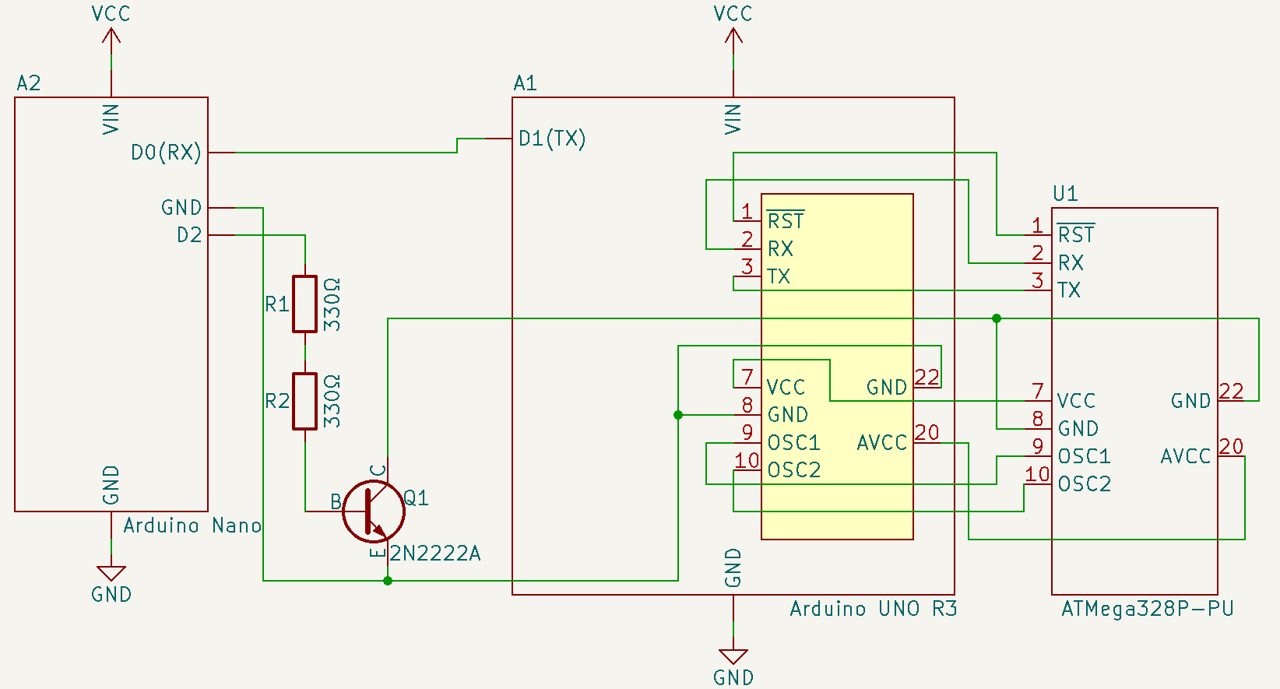
\includegraphics[width=1\textwidth]{images/schemeCTF.png}}
    \caption[Schéma zapojenia útoku na firmvér zo súťaže CTF]{Schéma zapojenia útoku na firmvér zo súťaže CTF \cite{vccOnTheCheap}. Žltý obdĺžnik znázorňuje púzdro na doske Arduio UNO, z ktorého bol vybratý mikrokontrolér ATMega328P.}
    \label{obr:schemeCTF}
\end{figure}

Ďalej je potrebné naprogramovať Arduino Nano, aby pomocou ovládania tranzistora na krátko odpojilo napájanie ATMega328P od zeme a následne opäť pripojilo. Dĺžka časového intervalu, počas ktorého je tranzistor vypnutý, musí byť dostatočne dlhá, aby indukovala chybu na procesore, ale nie príliš dlhá, aby sa mikrokontrolér resetoval. Vyskúšali sme do Arduino Nano nahrať program použitý aj v pôvodnom útoku \cite{vccOnTheCheap}, ktorý bol implementovaný v prostredí Arduino IDE. Algoritmus vypne tranzistor a vykoná niekoľko prázdnych iterácií for-cyklu, po ktorom tranzistor opäť zapne. Následne sa pokúsi prečítať výstup zo sériového portu na ATMega328P. V prípade, že sa podarí prečítať \uv{flag}, útok bol úspešný. V prípade, že sa \uv{flag} nepodarí prečítať, zväčší počet iterácií for-cyklu a postup zopakuje \cite{vccOnTheCheap}. Ukážka časti kódu, ktorá ovláda tranzistor, je v algoritme \ref{alg:vccOnTheCheap}.

\begin{lstlisting}[float,language=C,caption={Ovládanie tranzistora, ktorý spína napájanie na ATMega328P. Prevzaté zo zdrojového kódu pôvodného útoku \cite{vccOnTheCheap}.},label=alg:vccOnTheCheap]
int waste = 0;
digitalWrite(powerPin, LOW);
for (int i = 0; i<glitchDelay; i++){ waste++; }                    
digitalWrite(powerPin, HIGH);
glitchDelay += 10;
\end{lstlisting}

\subsection{Výsledok, analýza a vylepšenie útoku}
Útok bol vyskúšaný na štyri čipy ATMega328P. Na dvoch z nich (z rovnakej série výroby) sa útok úspešne podaril s podobným výsledkom ako v pôvodnom útoku \cite{vccOnTheCheap}. \uv{Flag} sa dokonca podarilo prečítať už pri nulovom počte iterácií for-cyklu, postačoval najkratší možný výpadok -- vypnutie a okamžité zapnutie tranzistora pomocou funkcie \uv{digitalWrite} z knižnice prostredia Arduino IDE. Na druhých dvoch exemplároch (z inej série výroby) útok nebol úspešný a aj pri tomto najkratšom možnom výpadku sa mikrokontrolér reštartoval. Rozhodli sme sa preto napätie na mikrokontroléri počas útoku podrobne analyzovať pomocou osciloskopu. Pre tento účel sme sa rozhodli ATMega328P zapojiť na kontaktom nepájivom poli bez dosky Arduino UNO. Schému a detaily tohto zapojenia sme popísali v kapitole \ref{kap:hardver}. Takéto zapojenie umožňuje jednoducho meniť zapojené elektronické súčiastky, čo poskytuje väčšiu flexibilitu vo voľbe parametrov týchto súčiastok pri analýze.

Pomocou osciloskopu sa podarilo určiť priebeh zmeny napätia na mikrokontroléri v čase s presnosťou na rádovo stovky nanosekúnd. Výsledkom bolo, že interval, počas ktorého nastalo podpätie bol príliš dlhý (približne 2 {\textmu}s), čo pri útoku na 2 čipy zo štyroch spôsobilo reštart mikrokontroléra. Ďalším zaujímavým pozorovaním bol fakt, že časový interval podpätia sa nepredlžoval so zväčšovaním počtu iterácií \uv{prázdneho} for-cyklu. Dôvodom môže byť optimalizácia kompilátora, ktorý sa oprávnene rozhodol zdanlivo \uv{zbytočný} for-cyklus odstrániť.

Doska Arduino Nano, ktorá ovládala tranzistor obsahuje tiež mikrokontrolér ATMega328P, s externým oscilátorom s frekvenciou 16 MHz. V kapitole \ref{kap:hardver} sme spomenuli ukážku nastavenia výstupnej logickej hodnoty na 1, resp. 0 pomocou jedinej inštrukcie SBI, resp. CBI. Tieto inštrukcie dokáže procesor vykonať počas dvoch taktov vďaka dvojfázovej pipeline (načítanie a vykonanie inštrukcie) \cite{atmegaData}. Pri frekvencii 16 MHz to znamená, že vypnutie a opätovné zapnutie tranzistora by teoreticky malo trvať 1/4 {\textmu}s. 

Rozhodli sme sa preto časti kódu, ktoré ovládajú tranzistor prepísať do jazyku asembler s využitím C Inline Assembly, ktorý je podporovaný aj kompilátorom prostredia Arduino IDE. Volania funkcie \uv{digitalWrite} sme teda nahradili ekvivalentnou konštrukciou pomocou inštrukcií SBI a CBI. Následne sme útok zopakovali s takto upraveným programom nahratým na Arduino Nano. Výsledkom bolo, že podpätie na mikrokontroléri trvalo približne 1/2 {\textmu}s, čo je štyrikrát menej ako predtým. Dlhší čas v porovnaní s teoretickým časom (1/4{\textmu}s), bol pravdepodobne spôsobený nenulovým reakčným časom tranzistora a vplyvom ďalších fyzikálnych faktorov. Pri takto krátkom čase už nenastal reštart žiadného z testovaných čipov, ale útok bol opäť neúspešný. Interval bol pravdepodobne príliš krátky a na žiadnom z čipov sa neprejavila chyba. Ďalej sme preto upravili kód napísaním vlastnej procedúry oneskorenia v asembleri (opäť s využitím C Inline Assembly). Procedúra pozostáva z inicializácie registra na kladnú hodnotu (osem-bitový parameter) a cyklu. V cykle postupne dekrementujeme tento register a následne vykonáme podmienený skok na začiatok cyklu, pokiaľ výsledok dekrementovania bol nenulový. Pseudokód procedúry v jazyku asembler uvádzame v algoritme \ref{alg:asmDelay}. Takáto procedúra umožňuje parametrizovať oneskorenie s presnosťou na trojice taktov (cyklus procedúry trvá tri takty). Po tejto úprave sa útok úspešne podaril na všetkých štyroch testovaných čipov. Útok bol zopakovaný niekoľkokrát (10--20), potrebné oneskorenia pre úspešný útok na každom z exemplárov sú zhrnuté v tabuľke \ref{tab:vccOnTheCheap2}. Väčšiu presnosť by bolo možné dosiahnuť pridaním presného počtu inštrukcií NOP, medzi vypnutím a zapnutím tranzistora. Počet inštrukcií NOP, by však musel byť známy v čase kompilácie, čo by znemožnilo dynamicky upravovať dĺžku oneskorenia za behu.

\begin{lstlisting}[float,language=C,caption={Procedúra oneskorenia v asembleri. \{IN\} označuje vstupný parameter -- 8-bitová konštanta, alebo hodnota v registri.},label=alg:asmDelay]
mov r24, {IN}   ; 1 takt
loop:
    dec r24     ; 1 takt
    brne loop   ; 2 takty pri vykonani skoku, 1 inak
\end{lstlisting}

\begin{table}
    \caption[Výsledky vylepšeného útoku zo súťaže CTF]{Výsledky vylepšeného útoku zo súťaže CTF. Každý riadok popisuje výsledok na jednom z čipov ATMega328P, na čipy zo série 2128BQY pôvodný útok nebol úspešný. Čísla v tabuľke udávajú vstupný parameter (počet cyklov) procedúry oneskorenia z algoritmu \ref{alg:asmDelay}.}
    \label{tab:vccOnTheCheap2}
    \begin{center}
    \begin{tabular}{|c|c|c|c|}
        \hline 
        Séria čipu & Min (úspešný útok) & Max (úspešný útok) & Ideál (úspešnosť nad 90\%) \\
        \hline
        2139E4A & 6 & 12 & 9--10 \\
        \hline
        2139E4A & 4 & 11 & 10 \\
        \hline
        2128BQY & 3 & 11 & 7 \\
        \hline
        2128BQY & 4 & 12 & 8--9 \\
        \hline
    \end{tabular}
    \end{center}
\end{table}

\section{Analýza zapojenia s tranzistorom}
Rozhodli sme sa ďalej podrobnejšie analyzovať priebeh napätia na mikrokontroléri medzi vypnutím a zapnutím tranzistora v predošlom útoku. Pre tento účel sme napísali jednoduchý program, ktorý periodicky zapína a vypína tranzistor. Dĺžka časového intervalu medzi vypnutím a zapnutím tranzistora je nastaviteľná pomocou analógového vstupu z potenciometra. Dĺžku tohto intervalu budeme v tejto časti udávať v počtoch iterácií procedúry oneskorenia z algoritmu \ref{alg:asmDelay}, ďalej len počet iterácií oneskorenia. Tento program sme nahrali a spustili na Arduino Nano a zapojili sme ho spolu s mikrokontrolérom ATMega328P rovnako ako vo vylepšenej verzii útoku z predošlej časti. Na vstupný analógový pin dosky Arduino Nano sme zároveň pripojili potenciometer, aby ním bolo možné regulovať počet iterácií oneskorenia. Následne sme pomocou osciloskopu MDO4104C merali priebeh napätia na mikrokontroléri, pri rôznej dĺžke intervalu medzi vypnutím a zapnutím tranzistora. Ako sme očakávali, na mikrokontroléri periodicky vznikalo podpätie. Napätie počas vypnutého tranzistora však neklesalo prudko, ale pomaly konvergovalo k hodnote približne 2 V. Po zapnutí tranzistora sa napätie vrátilo (za čas približne 300 -- 500 nanosekúnd) na pôvodnú úroveň 5 V. Dôsledkom takéhoto priebehu bol fakt, že pri kratších intervaloch medzi vypnutím a zapnutím tranzistora napätie nestihlo klesnúť ani pod hladinu 4 V, čo už priebeh programu na cieľovom ATMega328P neovplyvnilo.

Rozhodli sme sa preto ku GND pinu mikrokontroléra pripojiť zdvíhací odpor. Tento odpor, by po vypnutí tranzistora mal podvihnúť napätie medzi zemou a pinom GND, čím zmenší napätie medzi napájacími pinmi mikrokontroléra postupne až k nule (VCC aj GND sa vyrovnajú na 5 V). Vyskúšali sme rôzne hodnoty zdvíhacieho odporu, pričom sme pozorovali, že efekt zdvíhacieho rezistora sa zväčšoval so zmenšujúcou sa hodnotou jeho odporu. Čím menší bol odpor, tým väčšie podpätie sa počas krátkeho výpadku podarilo dosiahnuť. Až pri hodnote 330 $\Omega$ sme pozorovali značné zrýchlenie poklesu, čo je pomerne nízka hodnota na zdvíhací odpor. Nevýhodou je potom fakt, že pri zapnutom tranzistore rezistorom preteká pomerne veľký prúd (5 V/330 $\Omega$ = 15 mA), čo sa prejavilo citeľným zahriatím odporu počas experimentu. Na obrázku \ref{obr:vccAnalysis} je porovnaný priebeh napätia na mikrokontroléri s a bez použitia zdvíhacieho odporu zaznamenaný pomocou osciloskopu.

\begin{figure}
    \centerline{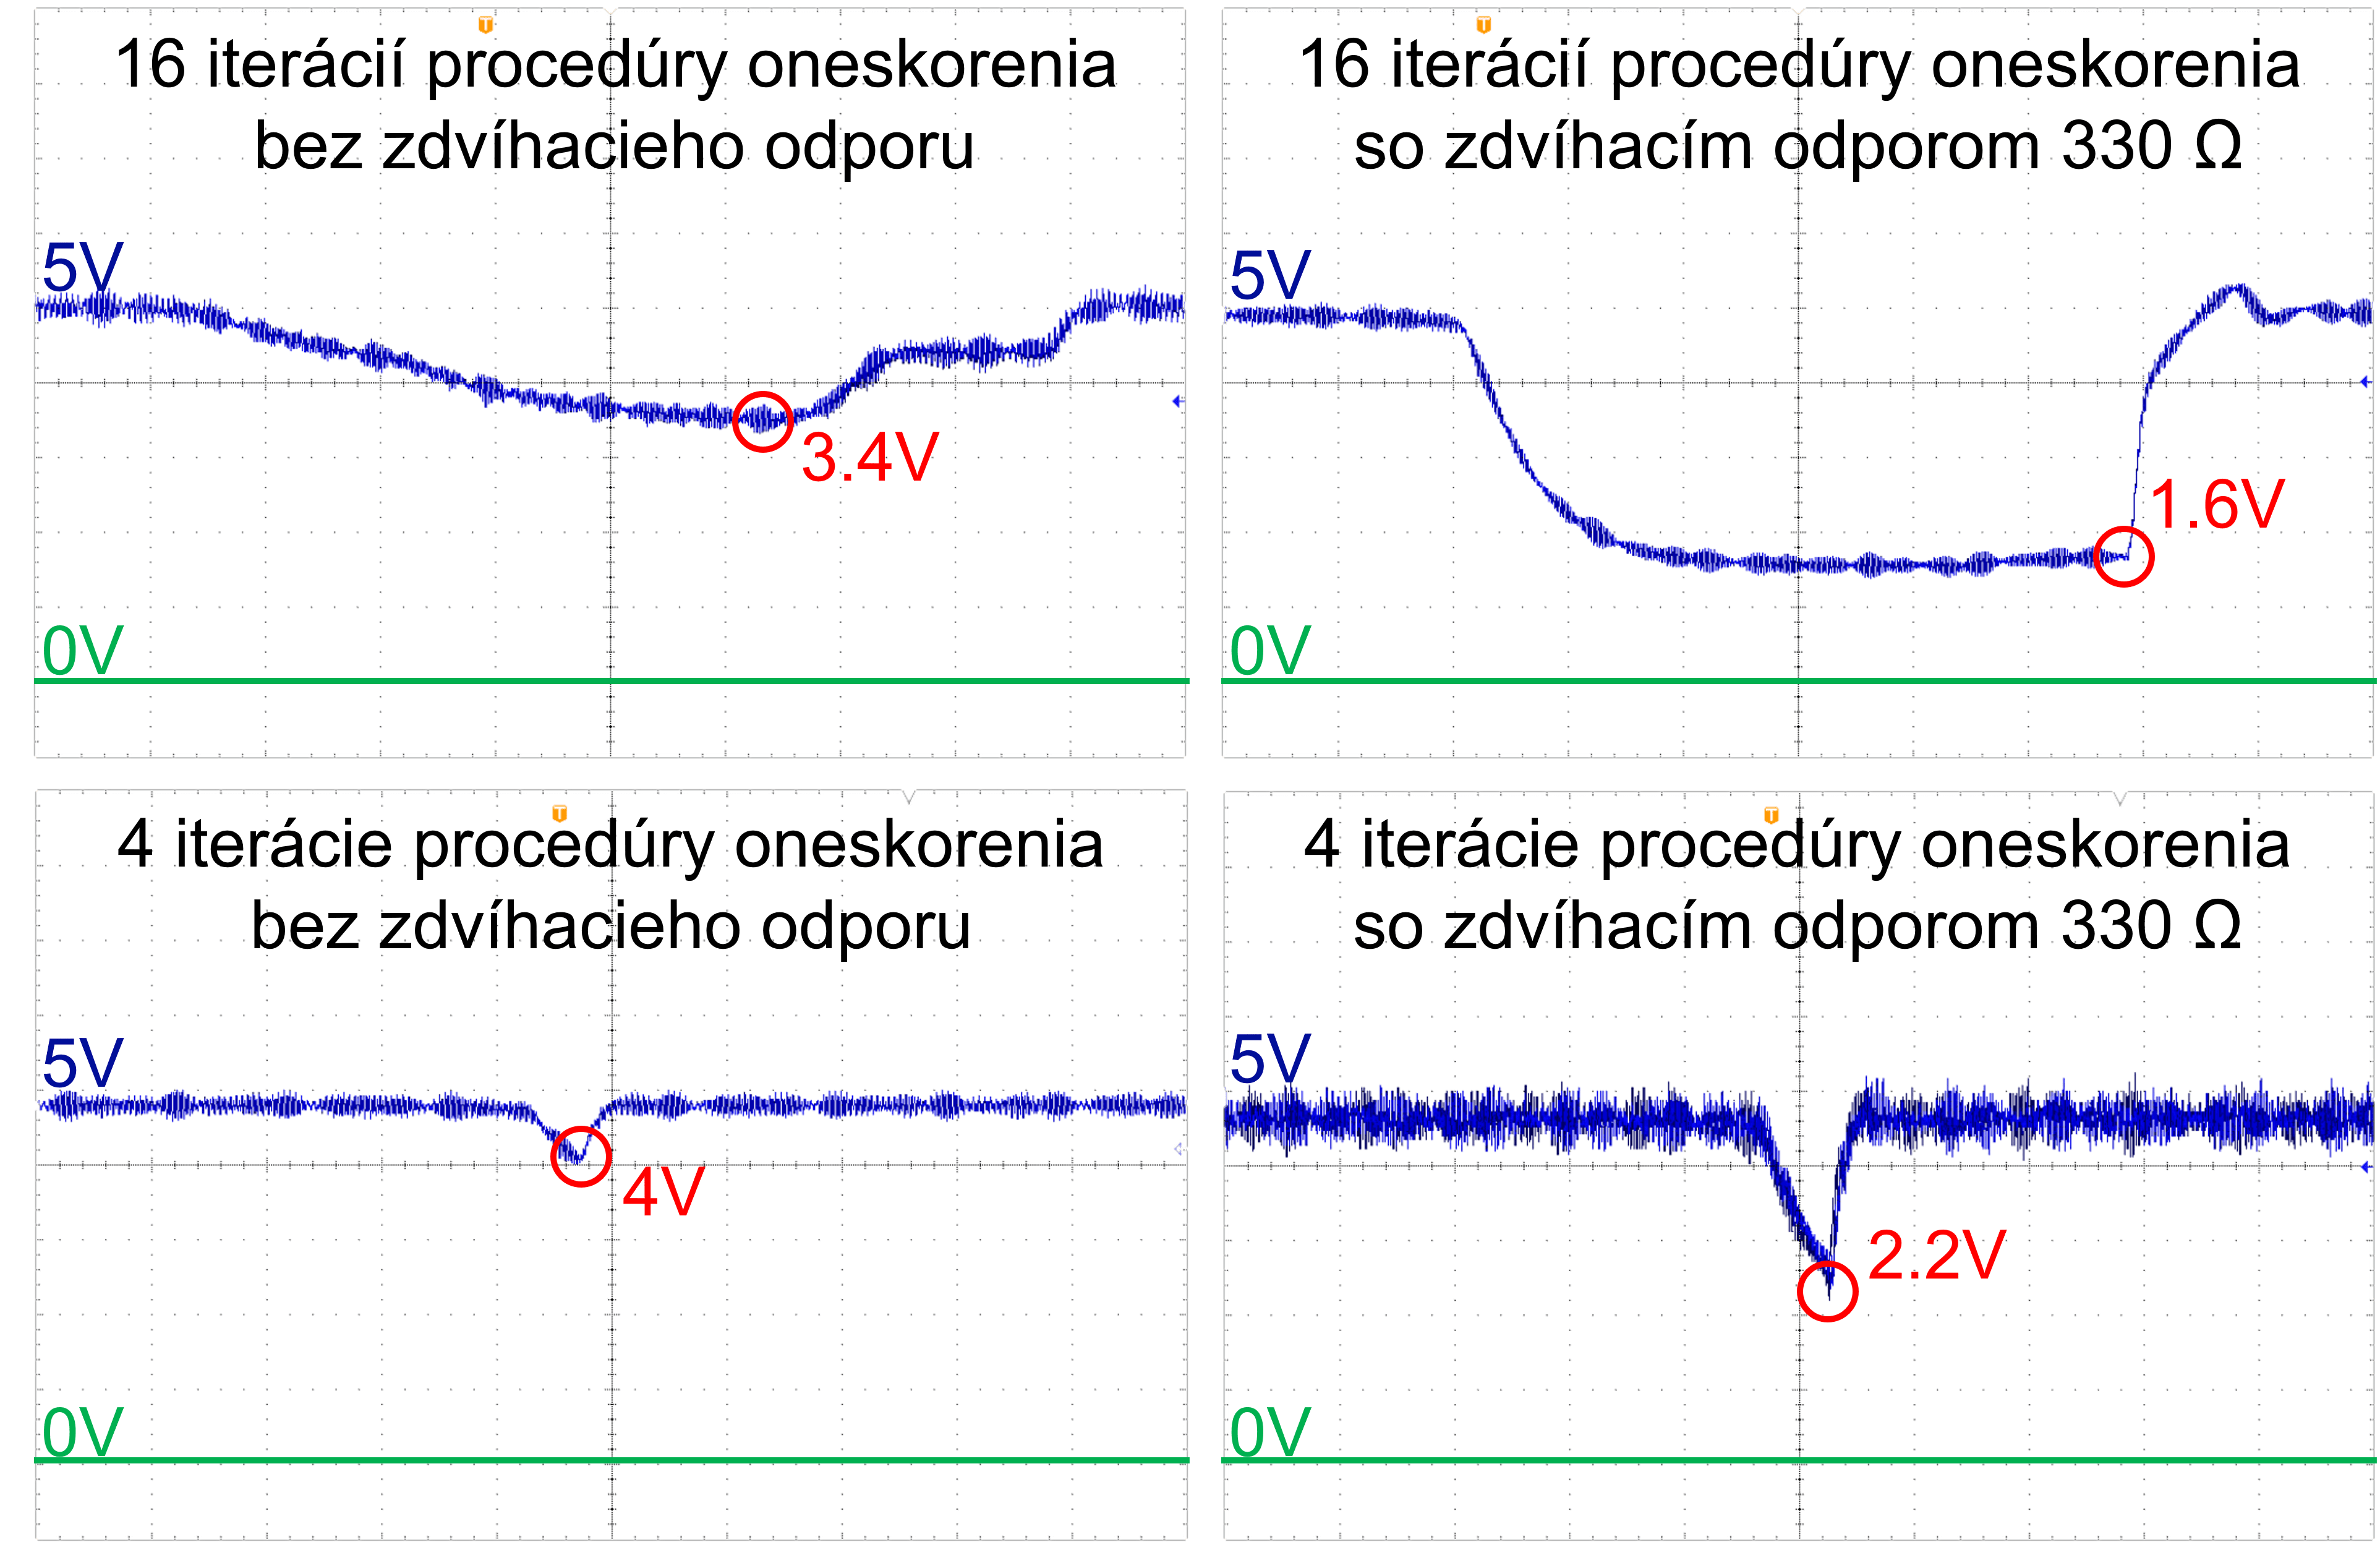
\includegraphics[width=1\textwidth]{images/vccAnalysis.png}}
    \caption[Porovnanie napätia na mikrokontroléri s/bez zdvíhacieho odporu]{Porovnanie napätia na mikrokontroléri s/bez zdvíhacieho odporu počas vypnutia tranzistora pri rôznom počte iterácií procedúry oneskorenia z algoritmu \ref{alg:asmDelay}. Veľkosť horizontálneho dielika je 400 ns. Použitý tranzistor je 2N2222A, zdvíhací odpor má hodnotu 330 $\Omega$. Modrou farbou je znázornená hodnota napätia v čase a zelená čiara v spodnej časti snímok označuje úroveň napätia 0 V. Červenou je zvýraznená minimálna nameraná hodnota napätia (zaokrúhlená na desatiny voltov).}
    \label{obr:vccAnalysis}
\end{figure}

Ďalej mohli byť príčinou takéhoto priebehu aj parametre tranzistora, ale aj niektoré pasívne súčiastky v zapojení. Rozhodli sme sa preto pozorovať ako použitie rôznych tranzistorov ovplyvňuje priebeh napätia na mikrokontroléri medzi vypnutím a zapnutím tranzistora. Vyskúšali sme tri rôzne bipolárne (BJT) tranzistory -- dva typu NPN aj jeden PNP. Aby bolo možné použiť tranzistor typu PNP, bolo potrebné mierne modifikovať zapojenie. Zmena spočíva v tom, že tranzistorom budeme odpájať napájací pin, miesto zeme, čo zároveň znamená, že miesto zdvíhacieho odporu použijeme uzemňovací (s rovnakým cieľom). Okrem toho vstup do bázy, ktorý riadi tranzistor bude obrátený (logická nula zapne tranzistor). Na obrázku \ref{obr:npnVpnp} je znázornený rozdiel medzi zapojením s tranzistorom typu NPN a PNP.

\begin{figure}
    \centerline{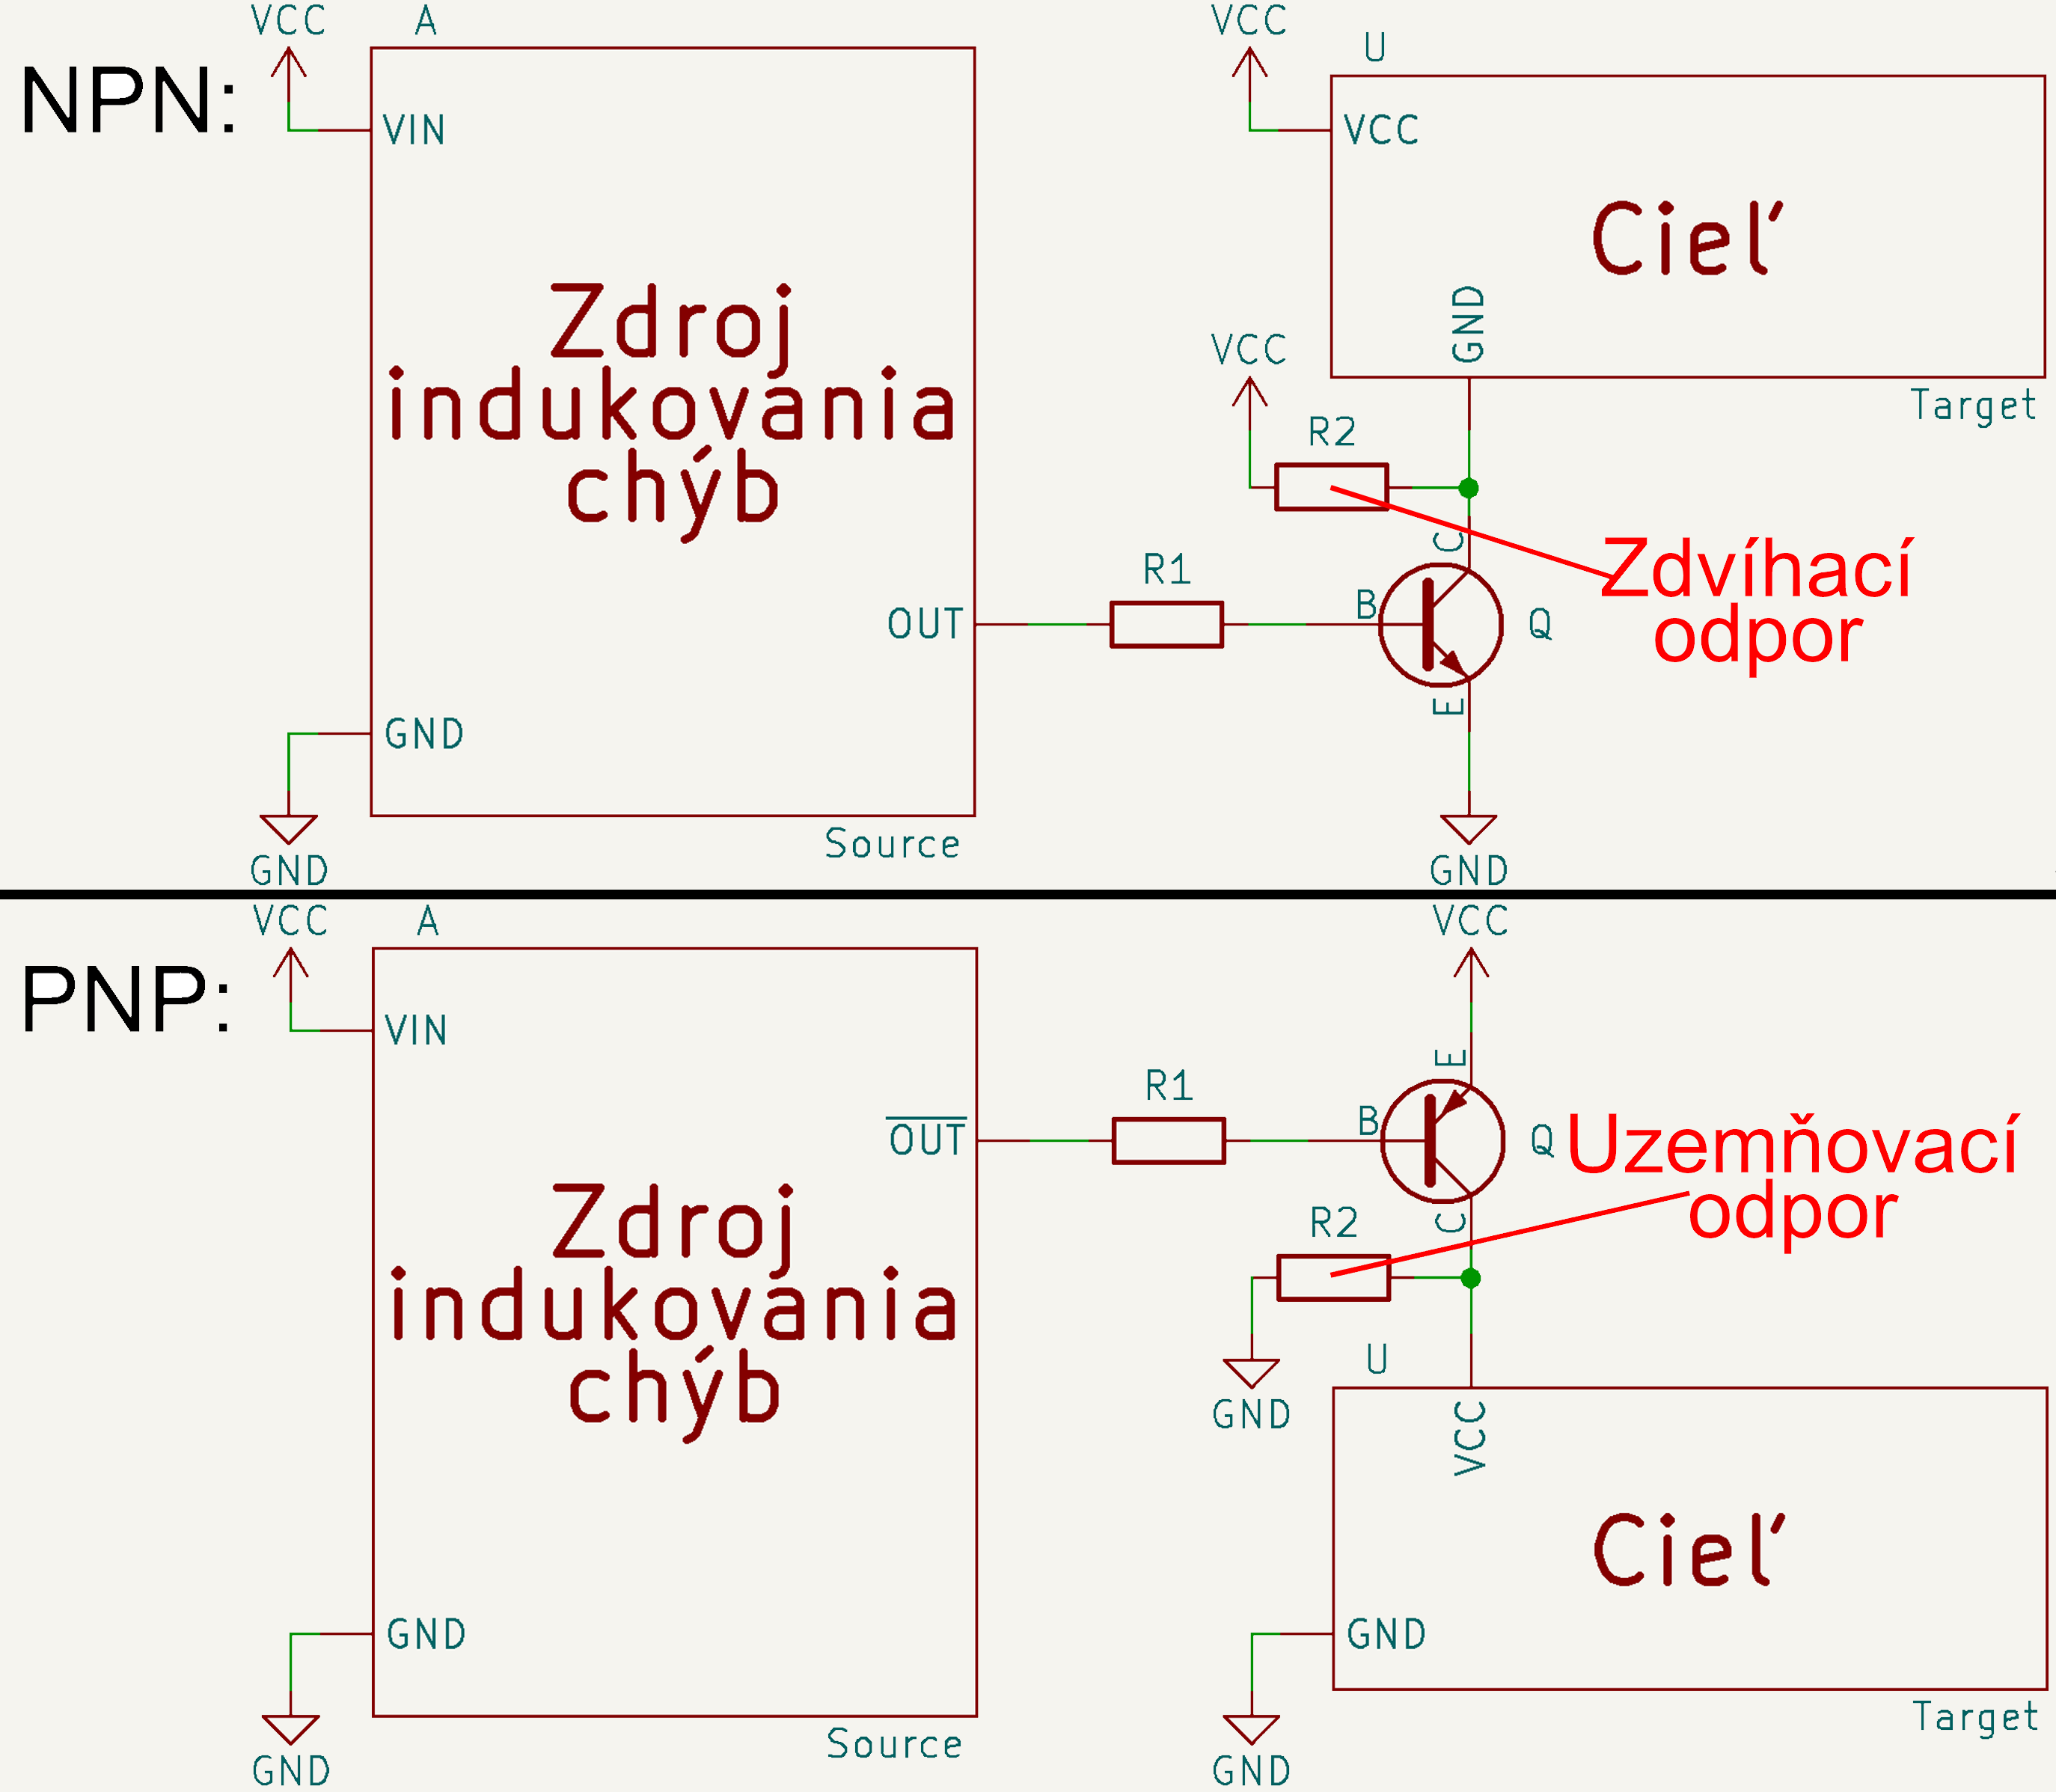
\includegraphics[width=0.8\textwidth]{images/npnVpnp.png}}
    \caption[Všeobecná schéma zapojenia s tranzistorom typu NPN a PNP]{Všeobecná schéma zapojenia s tranzistorom typu NPN a PNP.}
    \label{obr:npnVpnp}
\end{figure}

Zároveň sme každý tranzistor vyskúšali s rôznymi hodnotami zdvíhacieho, resp. uzemňovacieho odporu. Výsledky meraní sú zhrnuté v tabuľke \ref{tab:oscVoltage}, pričom \uv{víťazom}, ktorého sme sa rozhodli ponechať v zapojení pri ďalších útokoch bol tranzistor 2N2222A (NPN) so zdvíhacím odporom 330 $\Omega$ Tranzistor SS8050 mal síce kratšie časy stúpania a klesania napätia, ale minimálna úroveň napätia pri zapojení s 2N2222A bola nižšia. Dôvodom zvolenia veľmi nízkeho zdvíhacieho odporu 330 $\Omega$ bol fakt, že pri väčšom odpore bol rozdiel oproti zapojeniu bez zdvíhacieho odporu relatívne zanedbateľný.

\begin{table}
    \caption[Porovnanie priebehu napätia pri zapojení s rôznymi tranzistormi]{Porovnanie priebehu napätia na mikrokontroléri pri zapojení s rôznymi tranzistormi. Hodnoty v tabuľke sú priemerom zo šesťdesiatich štyroch vzoriek -- automaticky nameraných a vypočítaných pomocou funkcie osciloskopu. Napätie je zaokrúhlené na desatiny voltov a časy sú zaokrúhlené na stovky nanosekúnd.}
    \label{tab:oscVoltage}
    \begin{center}
    \begin{tabular}{|c|c|c|c|c|c|}
        \hline
        \multicolumn{6}{|c|}{Tranzistor 2N2222A (NPN)} \\
        \hline 
        zdvíhací odpor ($\Omega$) & žiaden & 10k & 1k & 330 & 220 \\
        \hline
        min úroveň napätia (V) & 3,4 & 3,3 & 2,6 & 1,6 & 1,5 \\
        \hline
        čas od vypnutia po pokles na úroveň 3 V (ns) & N/A & N/A & 1000 & 300 & 200 \\
        \hline
        čas od vypnutia po pokles na min úroveň (ns) & 2000 & 1800 & 1400 & 1000 & 900 \\
        \hline
        čas od zapnutia po návrat na úrovneň 5 V (ns) & 500 & 400 & 300 & 300 & 300 \\
        \hline
        \multicolumn{6}{|c|}{Tranzistor SS8050 (NPN)} \\
        \hline 
        zdvíhací odpor ($\Omega$) & žiaden & 10k & 1k & 330 & 220 \\
        \hline
        min úroveň napätia (V) & 2,6 & 2,5 & 2,2 & 1,8 & 1,5 \\
        \hline
        čas od vypnutia po pokles na úroveň 3 V (ns) & 1000 & 1000 & 500 & 300 & 200 \\
        \hline
        čas od vypnutia po pokles na min úroveň (ns) & 1800 & 1700 & 1000 & 900 & 900 \\
        \hline
        čas od zapnutia po návrat na úrovneň 5 V (ns) & 200 & 200 & 200 & 200 & 200 \\
        \hline
        \multicolumn{6}{|c|}{Tranzistor SS8550 (PNP)} \\
        \hline 
        zdvíhací odpor ($\Omega$) & žiaden & 10k & 1k & 330 & 220 \\
        \hline
        min úroveň napätia (V) & 3 & 2,9 & 2,7 & 2,1 & 2 \\
        \hline
        čas od vypnutia po pokles na úroveň 3 V (ns) & 1000 & 1000 & 700 & 400 & 300 \\
        \hline
        čas od vypnutia po pokles na min úroveň (ns) & 1000 & 1100 & 1000 & 1200 & 1200 \\
        \hline
        čas od zapnutia po návrat na úrovneň 5 V (ns) & 200 & 200 & 200 & 200 & 200 \\
        \hline
    \end{tabular}
    \end{center}
\end{table}

\section{Testovanie efektov vybraných útokov}
V tejto časti podrobnejšie preskúmame, čo presne sa dá útokom využívajúcim zapojenie analyzované v predošlej časti dosiahnúť. Pokúsime sa experimentálne určiť niektoré z možných efektov útoku na mikrokontroléri ATMega328P na úrovni makroinštrukcií procesora. Pomocou techniky zmeny napätia sa pokúsime ovplyvniť rôzne inštrukcie, prípadne kratšie časti kódu písané v jazyku asembler. Aby sme dosiahli väčšiu presnosť načasovania útoku, rozhodli sme sa pridať synchronizáciu medzi zariadením, ktoré ovláda tranzistor a mikrokontrolér, na ktorý útočime. ATMega328P zapojíme tak, ako sme popísali v kapitole \ref{kap:hardver} na kontaktnom nepájivom poli.